%\documentclass{sig-alternate}
%\documentclass[]{sig-alternate-05-2015}
%\documentclass[10pt, conference, compsocconf]{IEEEtran}
\documentclass[10pt, conference]{IEEEtran}
\IEEEoverridecommandlockouts      % enable the \IEEEpubid command for the 'conference' class

\usepackage{amsmath}
\usepackage{amsthm}
\usepackage{accents}
\newcommand*\underdot[1]{%
  \underaccent{\dot}{#1}}
\usepackage{mathtools}
\DeclarePairedDelimiter\ceil{\lceil}{\rceil}
\DeclarePairedDelimiter\floor{\lfloor}{\rfloor}
\usepackage{mathrsfs}
\usepackage{times}
\usepackage{multirow}
\usepackage{enumitem}
\usepackage{epsfig}
\usepackage{subfigure}
\usepackage{amsfonts}
\usepackage{amssymb}
\usepackage{graphicx}
\usepackage{url}
%\usepackage{cite}
\usepackage{psfrag}
\usepackage{array}
\usepackage{comment}
\usepackage{mdwmath} % part of Mark Wooding's powerful
\usepackage{mdwtab}  % tools for math, tables, ...
\usepackage{bm} % for the bold font Greek symbols in math mode
\usepackage{color}
%\usepackage[noend]{algorithmic}
\usepackage[noend]{algpseudocode}
\makeatletter
\usepackage{multirow}
\usepackage{algorithm}
\usepackage{xspace}
%\usepackage{flushend}  <-- Bear, ACM do not like balanced last page
\usepackage{natbib}  % for small reference font size
\def\bibfont{\footnotesize}
\setlength{\bibsep}{0.0pt}

%\usepackage{float}
%\usepackage{natbib}  % for small reference font size
%\def\bibfont{\scriptsize}
%\setlength{\bibsep}{0.0pt}
%\usepackage{enumitem}
%\setlist{nolistsep}

% INFOCOM specific space saving tips from Bo
%\renewcommand{\baselinestretch}{0.990}
% place it after 'documentclass' for shrinking line space. Default is 1. 0.92 is the minimum acceptable by INFOCOM
%\usepackage[left=0.625in,right=0.625in,top=0.75in,bottom=1in]{geometry}
% this sets the margins of the 3 sides. The numbers are the minimum acceptable by INFOCOM

\newtheorem{thm}{Theorem}
\newtheorem{cor}{Corollary}
\newtheorem{lem}{Lemma}
\newtheorem{dfn}{Definition}
\newtheorem{pbm}{Problem}
\newtheorem{claim}{Claim}

%\remove copyright box
%\makeatletter
%\def\@copyrightspace{\relax}
%\makeatother


\begin{document}
\sloppy

\title{
Streaming Scalable Video Sequences with Media-Aware Network Elements Implemented in P4 Programming Language
}

\author{ 
\IEEEauthorblockN{Chao-Wen Chen$^1$, Li-Wen Pan$^1$, Yu-Rong Wang$^1$, Ching-Ling Fan$^1$, and Cheng-Hsin Hsu$^1$}
\vspace{2pt}
\IEEEauthorblockA{$^1$Department of Computer Science, National Tsing Hua University, Taiwan}
}
\maketitle

\begin{abstract}
  We aim to reduce the negative impact of dropping packets inside the Internet. There are three drop logic are considered. (i) tail, (ii) enhancement-layer, and (iii) rate-distortion.
\end{abstract}
\begin{IEEEkeywords}
Scalable video streaming, media-aware network element, software-defined network, rate-distortion optimization
\end{IEEEkeywords}

\section{Introduction} \label{sec:introduction}

In recent years, people are getting used to rely on Over-The-Top (OTT) 
services such as Skype, Facebook, Youtube, Netflix, etc. 
Among these services, video streaming is one of the services which 
consumes the most network resources. Video streaming needs more and more bandwidth because receivers prefer higher video quality than before, and thus incur high traffic amount on the best-effort Internet. Turns out streaming high quality video with less network resources becomes much more important.

{\em Scalable Video Coding (SVC) }is one of solutions for network congestion. Each of the SVC sequences contains a header, a base and multiple enhancement layers. The header stores the information that how the decoder should recognize those packets, and the base layer consists the elementary information of that particular frame. Enhancement layers are all rely on the low layers to decode. For example, enhancement layer 1 can be decode only if receiver receive the base layer and enhancement layer 2 can be decode only if receiver receive the enhancement layer 1. Furthermore, the encoder will encode the discardability into the packetize header. Therefore, We can drop the discardable packets without affecting its decodability in the middle-box of the Internet. The dynamic decisions on which video packets to drop can be sub-optimally done by streaming servers or clients without the global knowledge of the Internet. The better way to approach is through {\em Media-Aware Network Elements (MANEs)}, which are switches with knowledge of packets header. However, changing the normal switches into MANEs is quite difficult and thus not likely to happen. Fortunately, with recent advances in {\em Software-Defined Networking (SDN)} and {\em Network Function Virtualization (NVF)}, network switches are much more programmable, and make collaborative MANEs into reality. 

In the following sections, we will introduce every tools we are going to use and evaluate the results of our experiments among each algorithm we designed.
\section{Programming Protocol-Independent Packet Processor} \label{sec:p4}

P4 is a programming language allows us to config a special design switch. In P4, we can tell the switch how to parse a packet by identifying the packet header. Furthermore, we can store or edit the content inside packet header and forward it to the right port or even drop it. 

\begin{figure}[tbh]
    \centering
    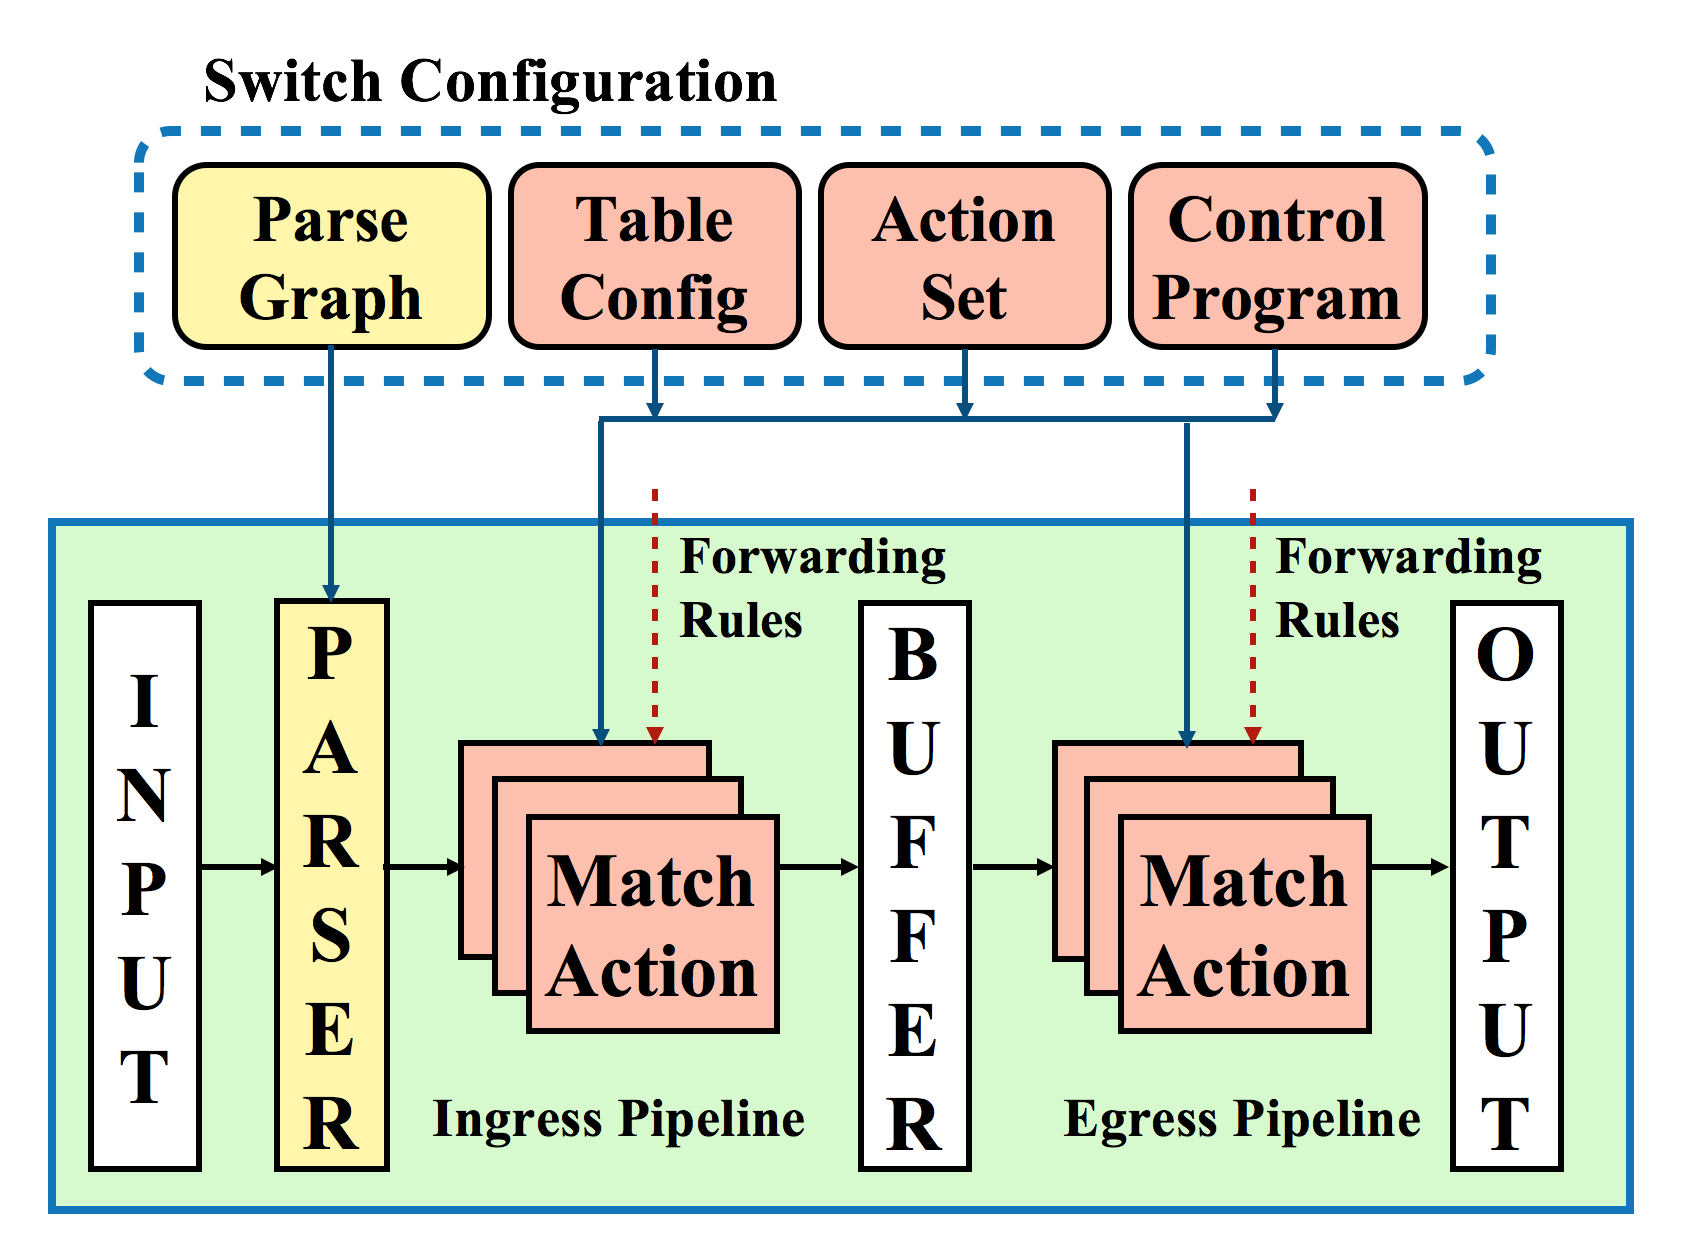
\includegraphics[width=.50\textwidth]{fig/p4.png}
    \caption{P4 Abstract~\cite{BDGI+14}}
    \label{p4}
\end{figure}

Fig.~\ref{p4} is a standard P4 switch diagram drawn by P4 Organization. Companies like Barefoot has designed some ASICs to run P4 program. It has many pipelines for us to deploy our P4 program in match and action table. P4 program actually consists of 4 parts, parse graph, table config, action set, control program. Parse graph tells P4 switch how to parse a packet. It could parse kinds of packets if we write it correctly. The other three parts works together. We have to implement many tables to match the field of packet header and actions. Each match+action table has a set of actions, we can match the packet to do the correction. The control program is more like a script exist both in ingress pipeline and egress pipeline. This control program will decide the order of math+action table. If the packet passes the two control pipeline, it will be pushed into output buffer and then send out by interface.
\section{Problem Definition} \label{sec:problemDefinition}

In modern network, we use Internet to deliver packets to exchange information all over the world. However, Internet is not designed for streaming videos or audios. The best-effort characteristic of Internet makes things become more complicated. Therefore, many experts had published many protocols and algorithms to make sure receiver can receive the whole data they are streaming and recover from packet loss. In our experiment, we use Scalable Video Evaluation Framework(SVEF) to stream our videos. In this framework, we stream videos based on UDP/IP network. In UDP protocol, sender will not receive any signal or ack to determine if receiver has already receive the packet or the packet is actually lost. With this characteristic, the sender can not know the condition of network or how to retransmit lost packets. In this situation, our goal is reduce or eliminate the undecodable packets or even select the packets with better quality and less packet size.

SVEF has already implemented the sender and receiver using socket programming in C language but it isn't using any further protocol such as RTP or RTSP to adjust sending rate or recover from packet loss. The sender of SVEF will first parse the trace file which we provide and build the packets of the whole video. In each video, header and base layer will be built into a single packet, and each enhancement layers will be pack into one packet. Then, it calculate the time gap between two frames as 1/fps. In this time gap, sender will try to send all the packets belong to that frame one by one and calculate the time it spend. If it costs less than the time gap, then it sleeps until the next time gap and transmit packets of next frame when time is up. On the other hand, sender will send an error message if it can not send all packets belong to that frame in the time gap. If that happens, it will cut the current transmission and start the next one.
\section{Related Work} \label{sec:relatedWork}

There are already many people make some interesting researches and experiments. For example, ~\cite{ruia2016flowcache} design a system.
\section{Drop Logics} \label{sec:dropLogics}

In our system, we implement a MANE in P4 language between hosts. As we mention before, our goal is to ensure the decodablity of each packet or even select the packets with higher quality. We tend to achieve this goal by dropping packets that are not important, which means they may cause network condition and also cannot decode in receiver host. We design three drop logics and streaming real video to achieve this goal. The three drop logics are (i) tail, (ii) EL, and (iii) RDO. 

\begin{algorithm}
    \begin{algorithmic}[1]
        \Procedure{Tail}{}
        \If {$qLen > qT$} \text{drop next packet}
        \Else \ \text{forward this packet}
        \EndIf
        \EndProcedure
    \end{algorithmic}
\end{algorithm}

Tail logic is the most easiest logic and it is similar to regular switches. We set a threshold, $qT$, to drop packets before the buffer in MANE is totally full. It's like a simple typical pure Random Early Detect(RED) method. However, even with RED, we cannot control which packet to send or drop. This can reduce the opportunity of network condition but it still forward undecodable packets and cause bandwidth waste.

\begin{algorithm}
    \begin{algorithmic}[1]
        \Procedure{Enhancement Layer (EL)}{}
        \If {$qLen > qT_3$} \text{drop Layers 1,2,3}
        \Else 
            \If {$qLen > qT_2$} \text{drop Layers 2,3}
            \Else 
                \If {$qLen > qT_1$} \text{drop Layers 3}
                \Else \ \text{forward this packet}
                \EndIf
            \EndIf
        \EndIf
    $qT_3\ > qT_2\ > qT_1$
        \EndProcedure
    \end{algorithmic}
\end{algorithm}

In EL logic, we set three thresholds which are $qT_3$, $qT_2$, and $qT_1$. When the size of queue exceed one of the threshold, we drop more packets. We start with the highest threshold, $qT_3$, the network condition is very bad if the size of queue exceeds this threshold. Therefore we have to drop most of the packets. Here we drop all the packets belong to enhancement layer. On the other hand, if the size of queue only exceed lower threshold. That means the network condition is not that bad and we can forward more packets. Through this approach, we eliminate undecodable packets. The result of experiments will present in the following sections.

\begin{algorithm}
    \begin{algorithmic}[1]
        \Procedure{Rate Distortion Optimize (RDO)}{}
        \If {$qLen > qT_3$}
        $drop\ if\ \dfrac{quality}{packetLen}\ <\ rT_3$
        \Else 
            \If {$qLen > qT_2$}
            $drop\ if\ \dfrac{quality}{packetLen}\ <\ rT_2$
            \Else\If {$qLen > qT_1$}
                $drop\ if\ \dfrac{quality}{packetLen}\ <\ rT_1$
                \Else \ \text{forward this packet}
                \EndIf
            \EndIf
        \EndIf
        
    \Comment{$qT_3\ > qT_2\ > qT_1$}
    \Comment{$rT_3\ > rT_2\ > rT_1$}
        \EndProcedure
    \end{algorithmic}
\end{algorithm}

To use RDO, first we have to calculate the value we want to compare, quality/packetLen. We use the reference software, JSVM, to encode h.264 file for streaming. While encoding the h.264 file, we record the PSNR value of each layer of each frame. Then we calculate the difference of PSNR value of each layer and divide with the length of packet. This leads to a new value, RDO value, which we use to determine to drop that packet. Then we will write this value into the trace file to packetize this information into every packet. If we want to stream the video which provides more quality and use less bandwidth. In this scenario, the RDO value represents the importance level of that packet. Our MANE should be able to parse that value and select reserve bandwidth for packets with higher RDO value.


\section{Behavior Model V2} \label{sec:bmv2}


Before we start to introduce our experiment system setup. We want to introduce the behavior model we use. Bmv2~\cite{bmv2} is a software switch recommended by p4.org and ONF. It is still in develop stage but already support many protocols such as P4 runtime, grpc protocol to accept commands and can be deployed different P4 program through SDN controller in runtime.

Bmv2 is an opensource software written in C++, and obey to P4 specification.
There are two versions of P4, P4-14 and P4-16, published in 2014 and 2016
 respectively. However, bmv2 does not only support P4-16. Version 2 means that they redesign this pervious behavior model. In behavior model, we have to recompile the whole program if we deploy a new P4 program. Fortunately, bmv2 fixed this problem and add some other fancy features. Now the P4 compiler will compile P4 program into JSON format and deploy into bmv2 without recompile it.

\begin{figure}[tbh]
    \centering
    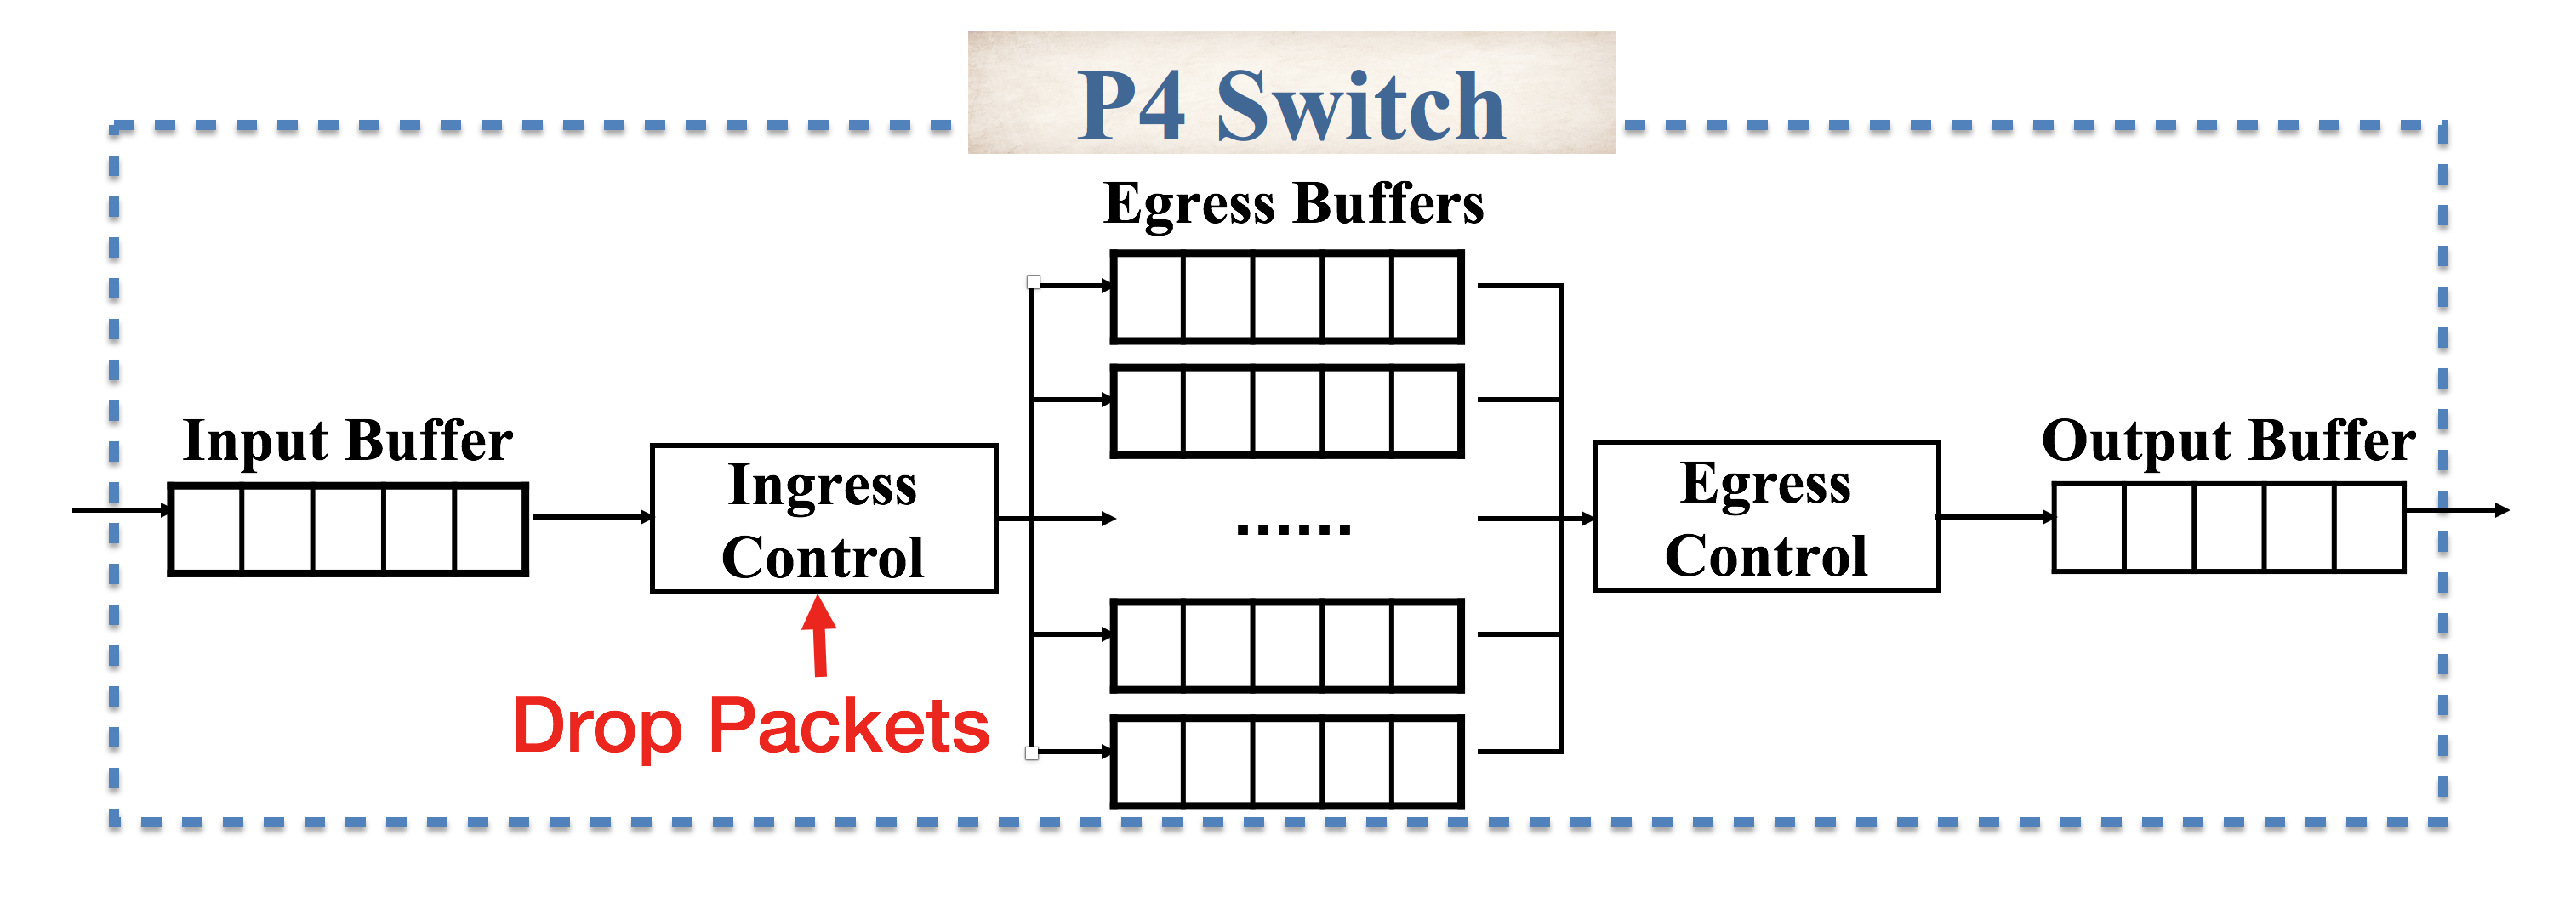
\includegraphics[width=.50\textwidth]{fig/bmv2Buffer.png}
    \caption{Buffers in bmv2}
    \label{bmv2Buffer}
\end{figure}

Fig. ~\ref{bmv2Buffer} shows all the buffer inside a bmv2. Please note that there are many interfaces connected to the buffer. Every packet comes into this MANE will first push into the input buffer. After our P4 program finish parsing the packet. Our ingress control will determine which port should this packet be forwarded and push into the right buffer relate to the port. In the ingress control, we detect the size of queue related to the forwarding egress buffer, and implement the three logics we mentioned before. If this packet pass the ingress control, it will be push into egress buffer and add some information such as source MAC address and reduce Time-to-Live value. Finally it will push to the interface attached to that port and leave MANE.



\section{Experiment Setup} \label{sec:setup}

We design a system using the tools we introduce above including SVEF, bmv2, and P4. Because of the limit of fund, we use bmv2 inside mininet and test our three drop logics. Three scenarios are designed to compare the difference among these drop logics. 

We use real H.264/SVC video sequences in our experiments, and these scenarios are done in mininet with software MANEs (running {\em bmv2}~cite{bmv2}) and virtual hosts.
In these scenarios, we would like to see the characteristic of P4 and our contribution. These three scenarios are described below:

Fig. ~\ref{scenario1}, ~\ref{scenario2} and ~\ref{scenario3} are scenarios we use to evaluate tail and EL logics. The RDO logic will be test only in scenario 3.

\begin{figure}[tbh]
	\centering
	\begin{minipage}[t]{0.24\textwidth}
	\centering
	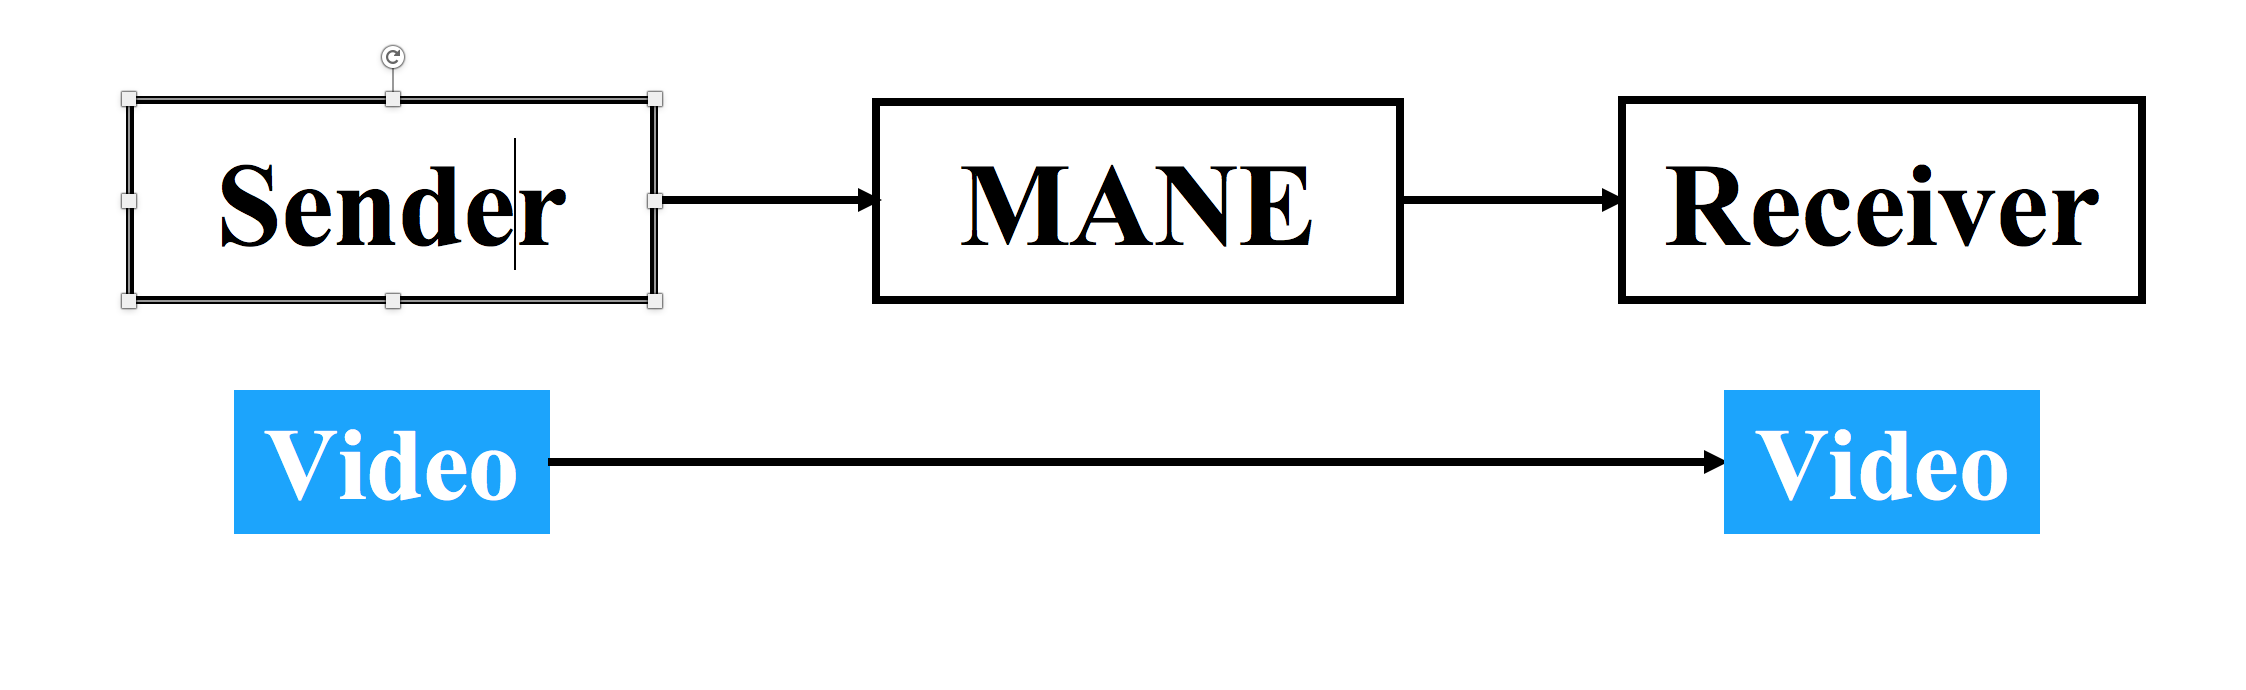
\includegraphics[width=\textwidth]{fig/scenario1.png}
	\caption{Testbed topology (scenarios 1).}
	\label{scenario1} 
	\end{minipage}
	\hfill\begin{minipage}[t]{0.23\textwidth}
	\centering
	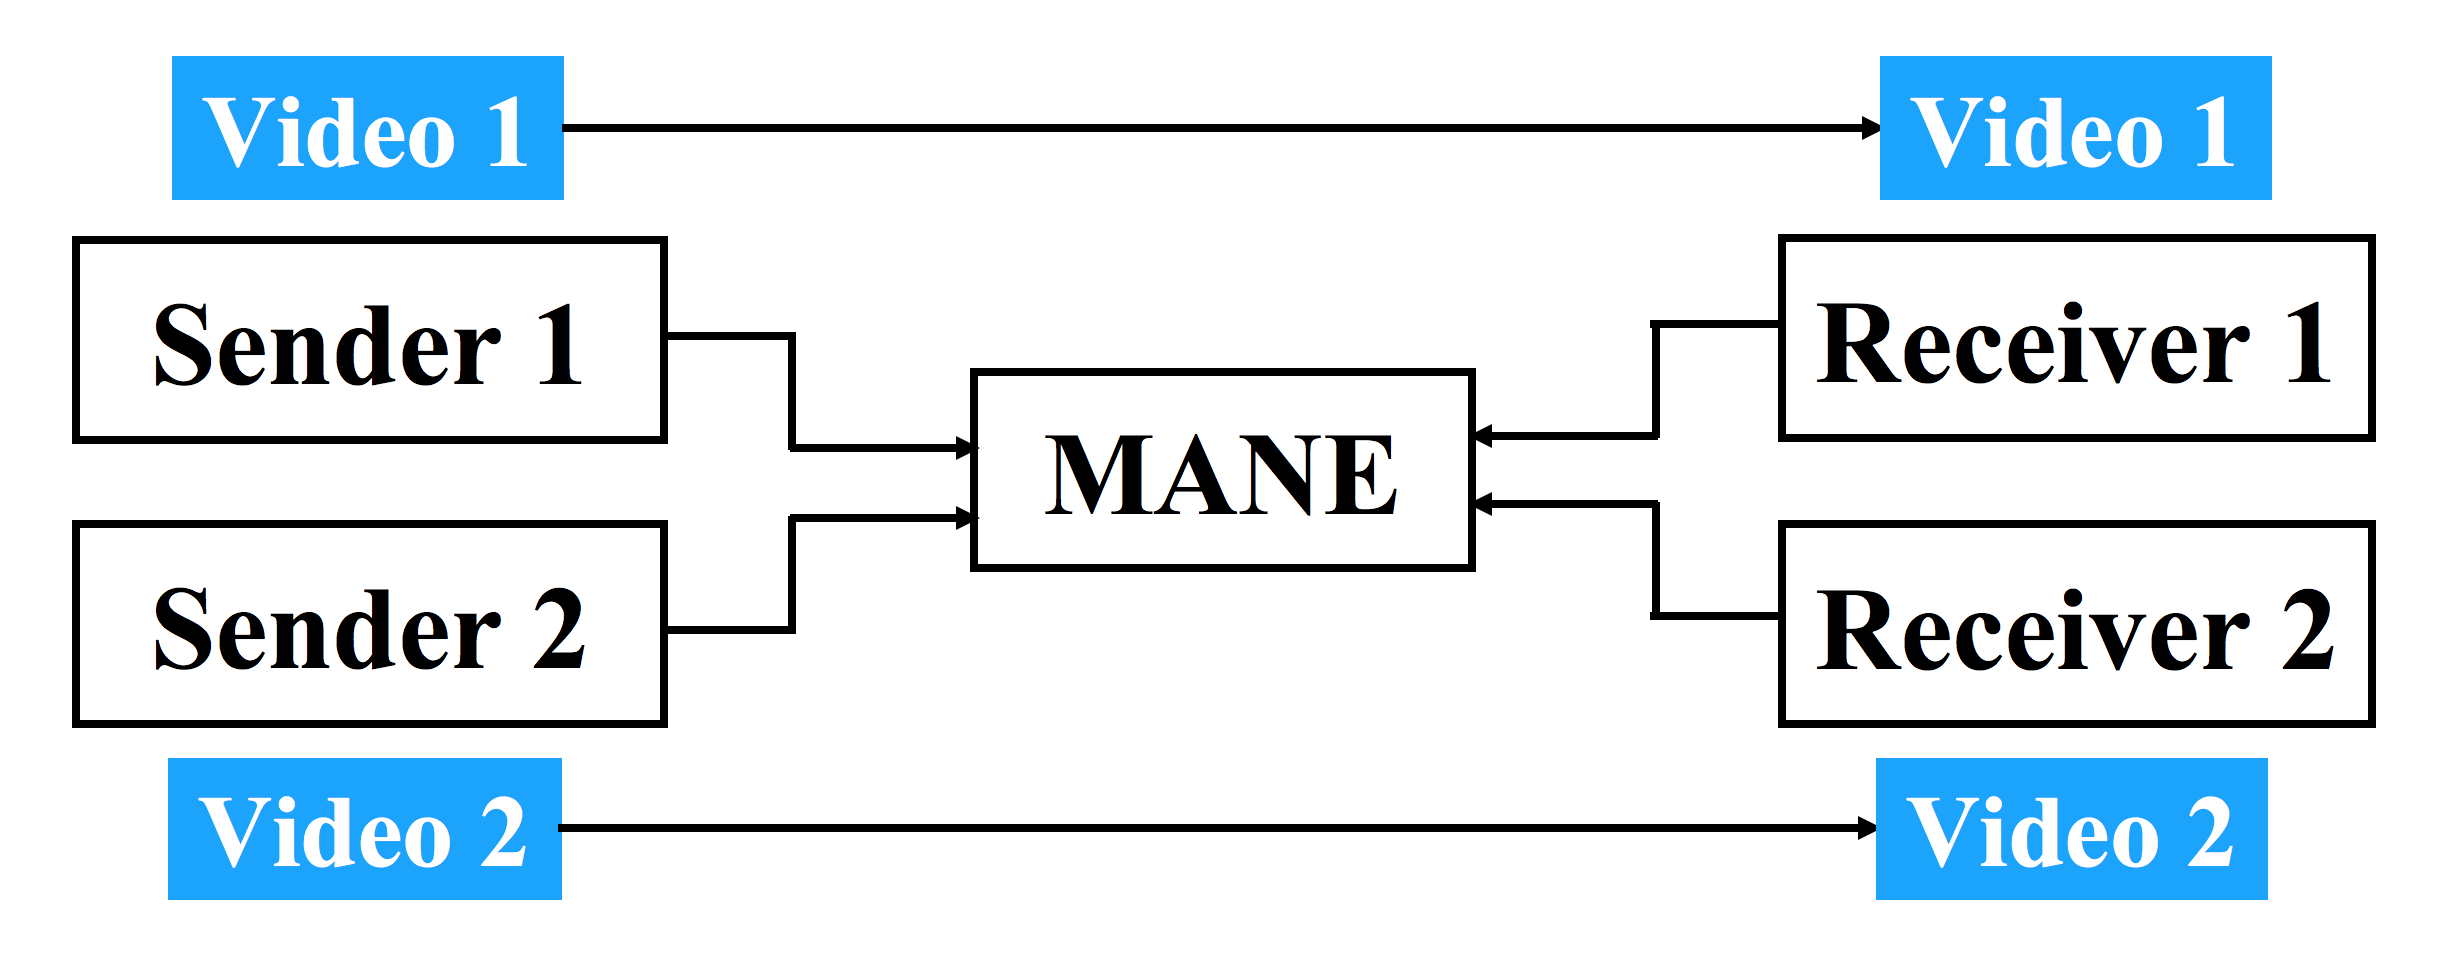
\includegraphics[width=\textwidth]{fig/scenario2.png}
	\caption{Testbed topology (scenario 2).}
	\label{scenario2} 
	\end{minipage}
	\vspace{-0.1cm}
\end{figure}

\begin{itemize} 
	\item {\bf Intelligent packet drops of a single video stream.}
	We construct a simple network with a sender, a controller, a MANE, and a receiver. Scenario 1 is the simplest topology. It consists of one sender and one receiver streaming one video. In this scenario, we want to observe the drawbacks of tail logic and see if EL logic can reduce network congestion by eliminate undecodable packets. The mininet bandwidth on the link is varied over time by scripts. In the MANE, we implement tail, EL, and RDO logics, and compare their performance. 

	\item {\bf Optimal packet drops across multiple video streams.}
	Scenario 2 is has four hosts with two sender and two receiver streaming two videos in mininet. In this scenario, we can use twice of buffer than scenario 1 because packets should be forwarded to different hosts and pushed into different buffer. In the MANE, we also implement three drop logics, and We can imagine that the result of scenario 1 and 2 would be very similar.

	\item{\bf Eliminate undecodable packets in less buffer}
	Scenario 3 shown in Fig.~\ref{scenario3} is the most challenging one. It contains one sender and one receiver streaming two videos in the same time. In this scenario, two streaming flows could affect each other since there is still exist a small time gap between them. When our P4-based MANE receive packets. It could push packets belong to one of the streaming flow but drop the other since the size of buffer exceed threshold after pushing that packet. 

\end{itemize}

\begin{figure}[tbh]
	\centering
	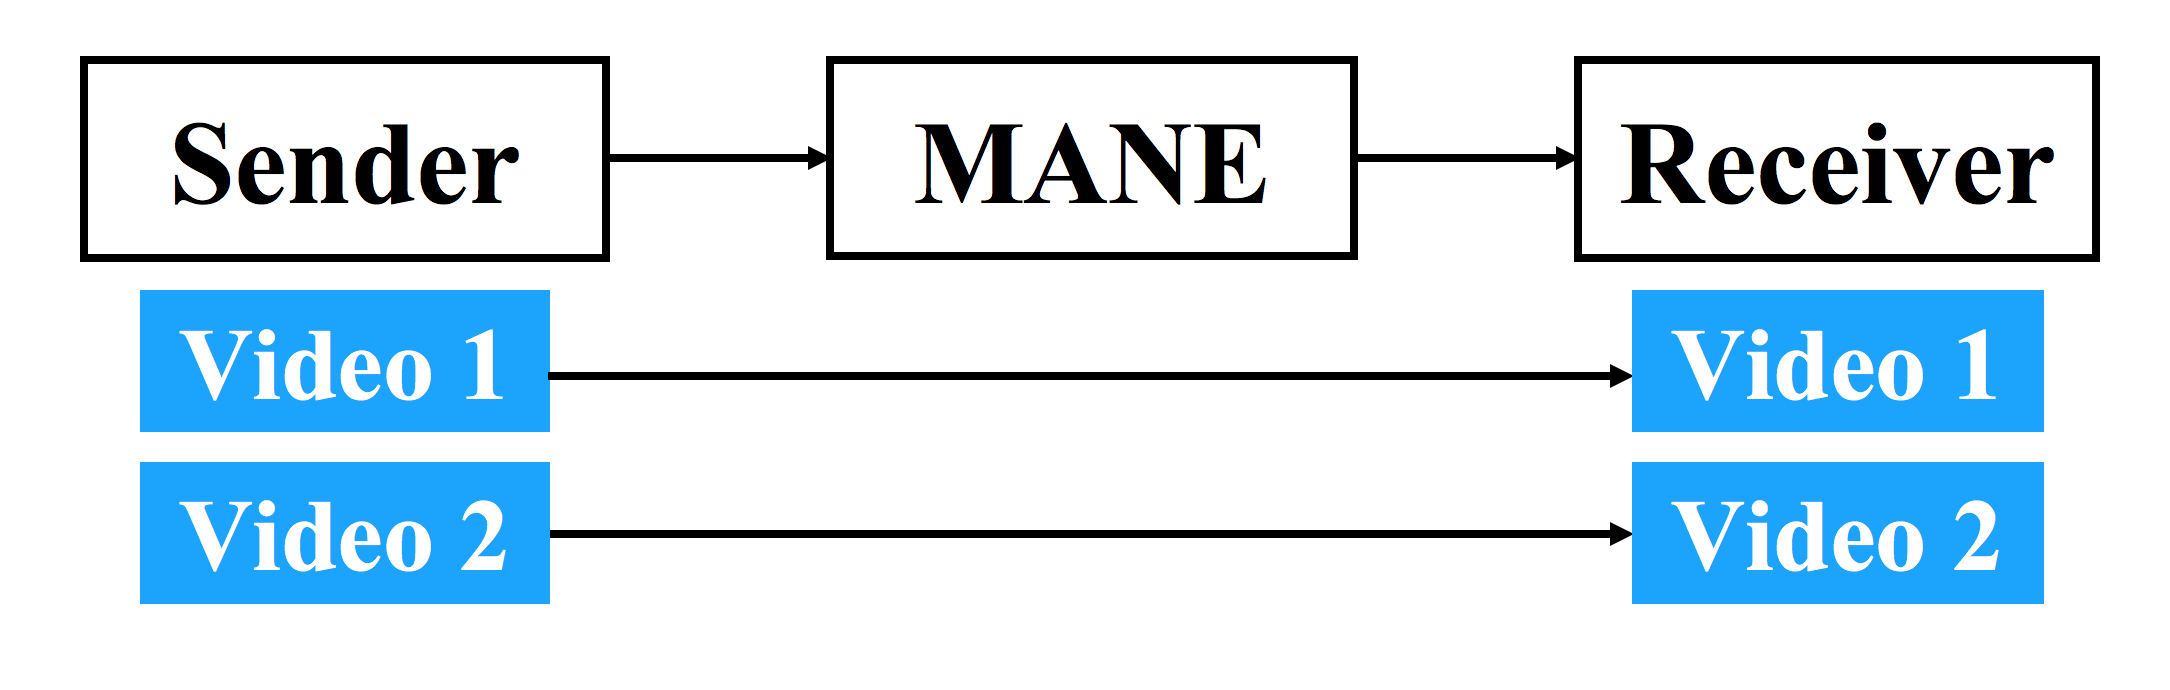
\includegraphics[width=.50\textwidth]{fig/scenario3.png}
	\caption{Testbed topology (scenarios 3).}
	\label{scenario3} 
\end{figure}

Among these scenarios. We try to limit the bandwidth between all of the links using tclink of mininet. However, this approach simply drops all packets at the backend of mininet if the throughput exceeds our administrate-set bandwidth without any signal or error exception. Even the bmv2 itself doesn't know if the packet is transmit by the attached interface. We follow the instructions given by the author of bmv2, limit the bandwidth by limit the packet sending rate. Through this approach, we can limit the bandwidth by quantities of packet instead of throughput. We need this because our drop logics will decide which packet to drop instead of dropping partition of the packet content.

%{\bf Preliminary evaluation.}
%To evaluate the performance of RDO, we use the following Quality of %Experience (QoE) measurements to compare tail drop, base-only and RDO %algorithms and compare the RDO with the general switches as well.

%\begin{itemize}
%\item {\bf Network latency}  Since more and more people watch video online, network latency is an important factor that impact users on watching videos.
%\item {\bf Network bandwidth} Videos nowadays usually have large resolutions, especially the presence of 4K videos. However, it is difficult to upgrade the network bandwidth on network links, which are usually fixed. Thus, we evaluate our algorithms and expect RDO can   
%\item {\bf Video quality}
%\end{itemize}

\section{Experiment Result} \label{sec:result}

We have use the three scenarios and three drop logics to run some experiments and gain significant improvement compared with tail and EL logic. In these experiments. We use uncompressed 4:2:0 YUV files to encode some 10 seconds videos. We adjust the packet process rate of MANE by time. The packet process rate starts slow and last for 3 seconds and is raised at the third second. Finally reduce to the slow start rate at the sixth second. 

\begin{subsection}
    {Scenario 1}

\begin{figure*}[tbh]
	\centering
	\begin{minipage}[t]{0.80\textwidth}
	\centering
	\includegraphics[width=\textwidth]{fig/tail_received_packets.eps}
	\caption{Result of Tail Logic in Scenario 1.}
	\label{tail_received_packets_S1} 
	\end{minipage}
	\hfill\begin{minipage}[t]{0.80\textwidth}
	\centering
	\includegraphics[width=\textwidth]{fig/EL_received_packets.eps}
	\caption{Result of EL Logic in Scenario 1.}
	\label{EL_received_packets_S1} 
	\end{minipage}
	\vspace{-0.1cm}
\end{figure*}


In Fig.~\ref{tail_received_packets_S1} and Fig.~\ref{EL_received_packets_S1}, the red part represents the packets that receiver has received. Each red box represent a packet except header and base layer, they are combined into a single packet. The y-axis from original point represents the header, base layer, enhancement layer 1,2,3, respectively. On the other side, x-axis represent the packets count. We can see that there are some gaps in Fig.~\ref{tail_received_packets_S1}. This is because the size of buffer exceeds our threshold then we drop every packet comes into the MANE. These gaps leads to a very bad watching experience. Receiver could decode the whole video but filling static frames into those gaps, and the video will stuck at these moments.

The EL logic gains a significant improvement. We can tell that there are no undecodable packets in Fig.~\ref{EL_received_packets_S1} and either any gap. In video streaming, we always want to maintain the quality of video. That means the quality or bitrate shouldn't shock severely. We can see EL logic achieves two goals, (i) eliminate undecodable packets and (ii) maintain the smooth sending rate.

\begin{figure}[tbh]
	\centering
	\begin{minipage}[t]{0.24\textwidth}
	\centering
    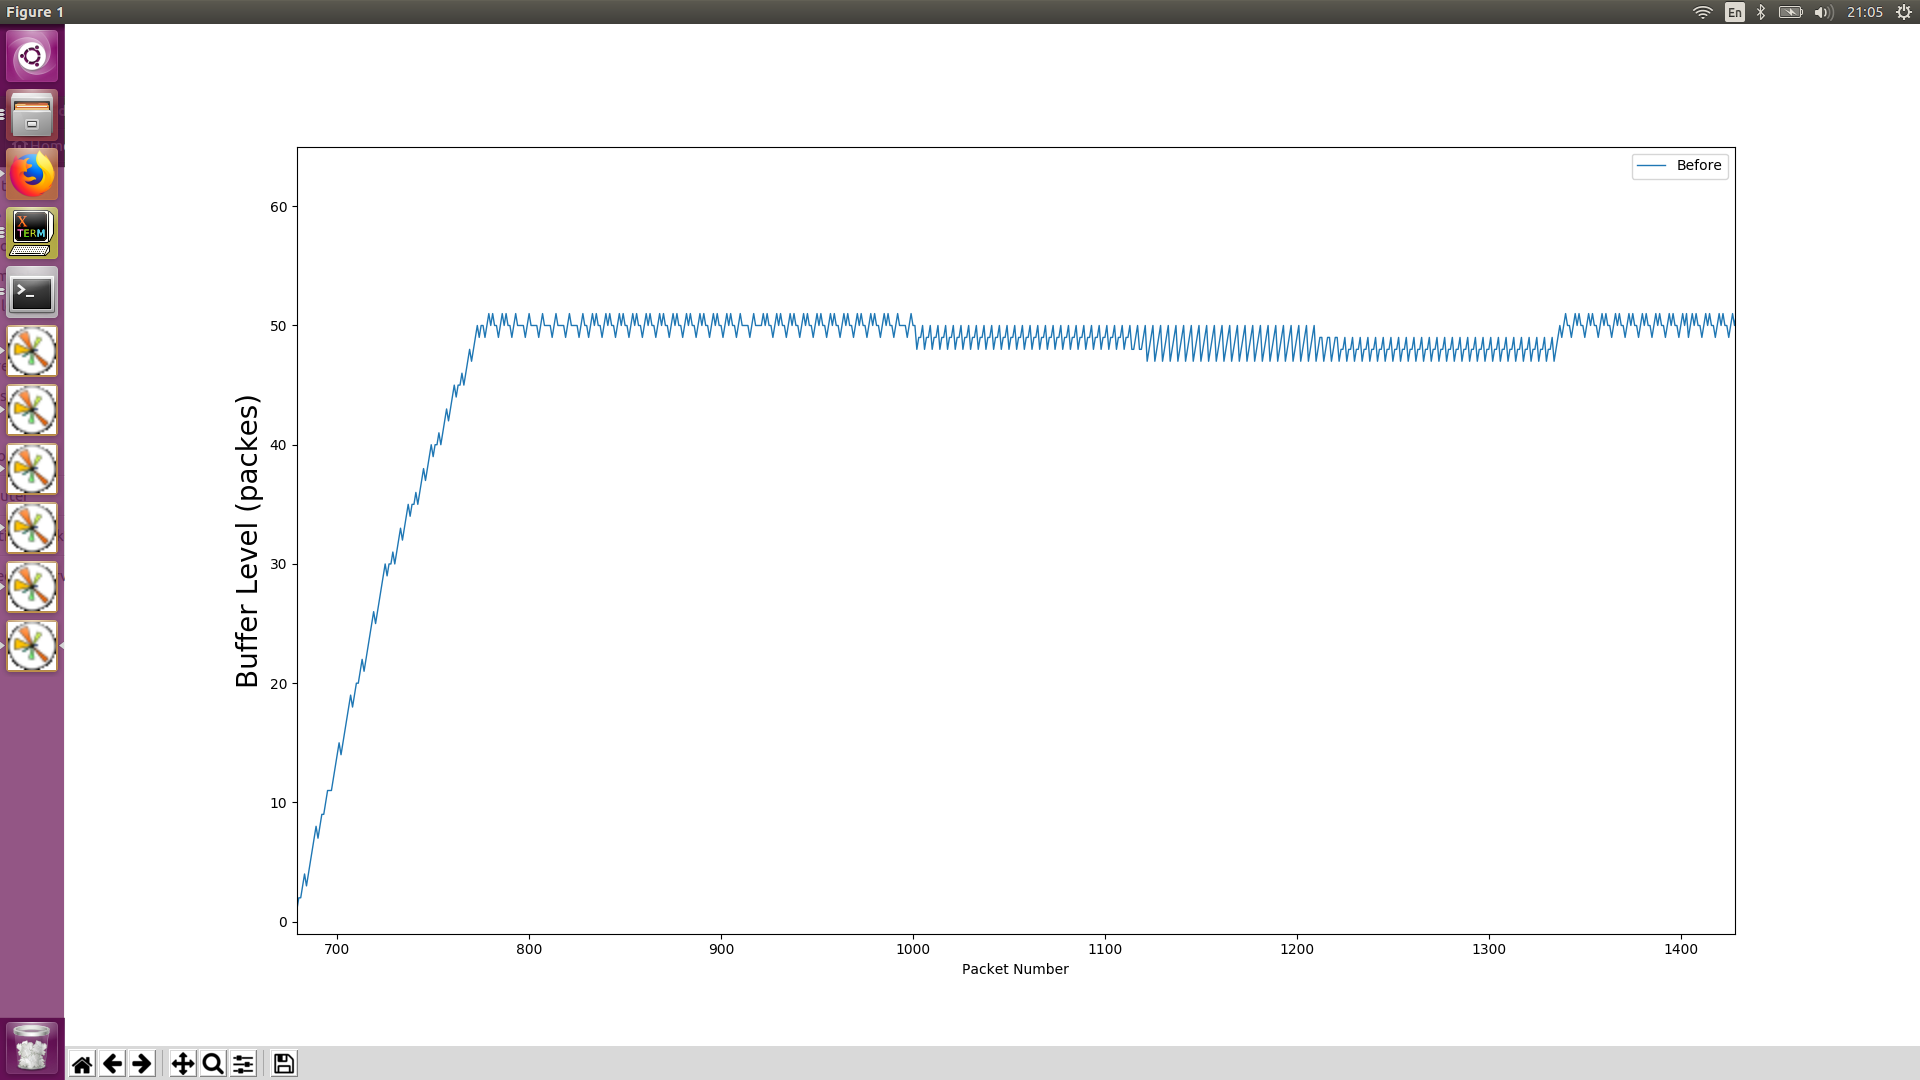
\includegraphics[width=\textwidth]{fig/tail_scenario1_buffer.png}
    %%%% figure needs to be changed %%%%%
	\caption{Buffer level of tail logic in scenario 1}
	\label{tail_scenario1_buffer} 
	\end{minipage}
	\hfill\begin{minipage}[t]{0.23\textwidth}
	\centering
	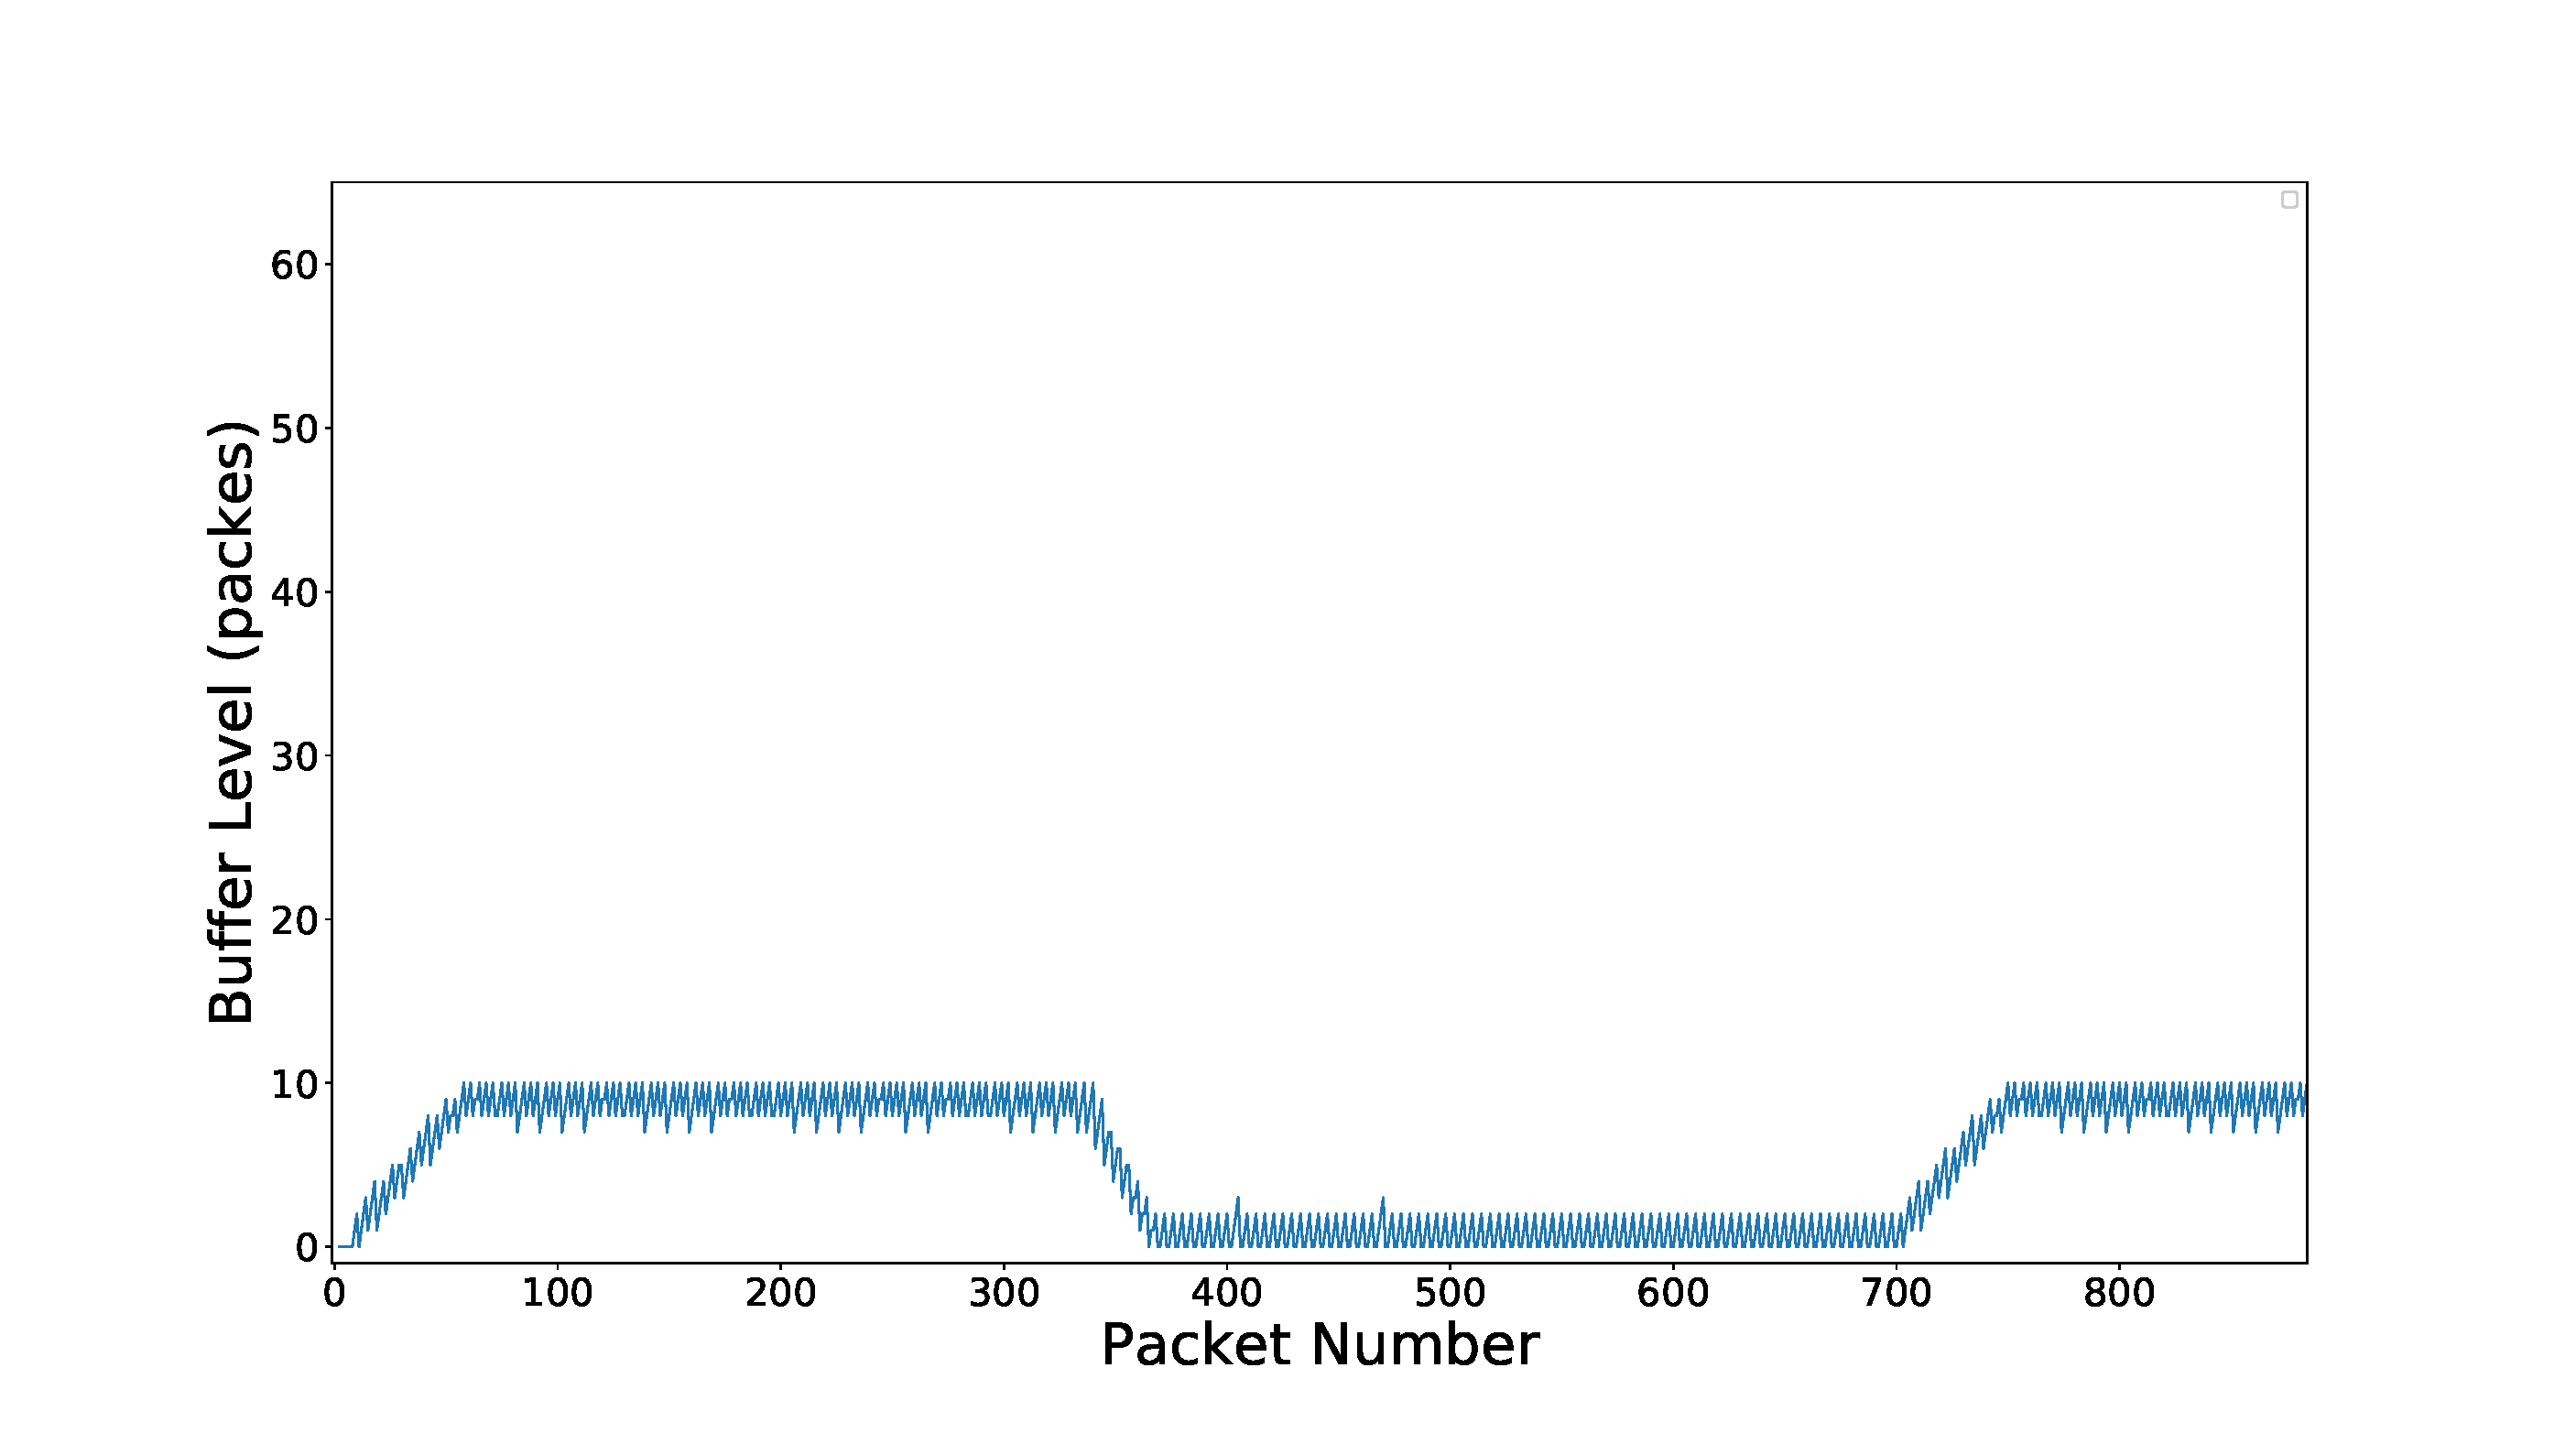
\includegraphics[width=\textwidth]{fig/EL_scenario1_buffer.eps}
	\caption{Buffer level of tail logic in scenario 1}
	\label{EL_scenario1_buffer} 
	\end{minipage}
	\vspace{-0.1cm}
\end{figure}

Despite of the result of received packets. We also plot the buffer level of each experiment. In these figures, x-axis represents the packets count and y-axis represents the quantities of packets inside the queue. We can observe that the buffer level of tail logic in scenario 1 in Fig.~\ref{tail_scenario1_buffer} grows up in the beginning and stop at 85\%, the threshold we set, and continue to the end of streaming. This is because we start to drop everything coming into our MANE.

Fig.~\ref{EL_scenario1_buffer} shows the buffer level of EL logic in scenario 1. We can observe that the buffer level also grows up in the beginning. However, it starts to drop some packets when the buffer level exceeds our threshold. In this scenario, the first threshold let MANE drops enough packets to maintain the buffer level. Then we raise the packet process rate of MANE, and buffer level goes down. Finally, it raise again because we reduce the packet process rate.
\end{subsection}
%%%%% change the figures %%%%%

\begin{subsection}{Scenario 2}

\begin{figure}[tbh]
	\centering
	\begin{minipage}[t]{0.24\textwidth}
	\centering
	\includegraphics[width=\textwidth]{fig/tail_received_packets.eps}
	\caption{Result of Tail Logic in Scenario 2. (Flow 1)}
	\label{tail_received_packets_S2_V1} 
	\end{minipage}
	\hfill\begin{minipage}[t]{0.23\textwidth}
	\centering
	\includegraphics[width=\textwidth]{fig/EL_received_packets.eps}
	\caption{Result of tail Logic in Scenario 2. (Flow 2)}
	\label{tail_received_packets_S2_V2} 
	\end{minipage}
	\vspace{-0.1cm}
\end{figure}

\begin{figure}[tbh]
	\centering
	\begin{minipage}[t]{0.24\textwidth}
	\centering
	\includegraphics[width=\textwidth]{fig/tail_received_packets.eps}
	\caption{Result of EL Logic in Scenario 2. (Flow 1)}
	\label{el_received_packets_S2_V1} 
	\end{minipage}
	\hfill\begin{minipage}[t]{0.23\textwidth}
	\centering
	\includegraphics[width=\textwidth]{fig/EL_received_packets.eps}
	\caption{Result of EL Logic in Scenario 2. (Flow 2)}
	\label{EL_received_packets_S2_V2} 
	\end{minipage}
	\vspace{-0.1cm}
\end{figure}

%%%%%

Fig.~\ref{tail_received_packets_S2_V1} and~\ref{tail_received_packets_S2_V2} shows the result of two streaming flows in scenario 2. Due to the characteristic of bmv2, we can use twice of buffer compare to scenario 1. Therefore we are actually doing the same thing as scenario 1 but do it twice. We can see that the result of flow 1 and flow 2 are almost the same. However, the tail logic sometimes performs very good or very bad. We assume it's because one of the flow occupy the network bandwidth so the other flow could not even get into the MANE or it arrives after the buffer level exceeds the threshold and leads to packet drop. In EL logic, we can see that results are also very similar. However, this result is much more stable. Even we run this experiment many times, the result doesn't change much. Since we have twice of the egress buffer, the result of the buffer level is also similar to scenario 1. Through this scenario, we can know how P4 specifies bmv2 to process packets and prove that using two buffers doesn't affect the efficiency of bmv2.

\end{subsection}

\begin{subsection}{Scenario 3}
    In Scenario 3, we stream two videos in the same buffer. Therefore, the results could be much worse than other scenarios. However, we still want to see the difference between tail and EL logics. Hence, we can observe if there are two video stream in the same buffer, how could RDO choose to stream.

    \begin{figure}[tbh]
        \centering
        \begin{minipage}[t]{0.24\textwidth}
        \centering
        \includegraphics[width=\textwidth]{fig/RDO_CREW.eps}
        \caption{Result of RDO Logic in Scenario 3. (Flow 1)}
        \label{RDO_received_packets_S3_V1} 
        \end{minipage}
        \hfill\begin{minipage}[t]{0.23\textwidth}
        \centering
        \includegraphics[width=\textwidth]{fig/RDO_ICE.eps}
        \caption{Result of RDO Logic in Scenario 3. (Flow 2)}
        \label{RDO_received_packets_S3_V2} 
        \end{minipage}
        \vspace{-0.1cm}
    \end{figure}

    In RDO logic, we want to maximize the total PSNR value of all video streams. This may lead to a unbalanced packet processing. In extreme examples, some videos provides little quality but cost much bandwidth. Therefore, RDO logic aims to choose the video packet provides higher quality and costs less bandwidth. To remark the result, we choose two videos one consists of many moving subject and another has many stable frames. We can see the results in Fig.~\ref{RDO_received_packets_S3_V1} and ~\ref{RDO_received_packets_S3_V2}. 

    Receiver of flow 1 receives 3.17 layers in average and flow 2 receives 2.81. Moreover, the average PSNR value are 33.17db and 29.33db \em{which means the quality is actually twice better than another.} The total average PSNR is ?? which is ?? higher compare to EL logic.

    %%%% change figures %%%%
    \begin{figure}[tbh]
        \centering
        \begin{minipage}[t]{0.24\textwidth}
        \centering
        \includegraphics[width=\textwidth]{fig/RDO_CREW.eps}
        \caption{Result of tail Logic in Scenario 3. (Flow 1)}
        \label{tail_received_packets_S3_V1} 
        \end{minipage}
        \hfill\begin{minipage}[t]{0.23\textwidth}
        \centering
        \includegraphics[width=\textwidth]{fig/RDO_ICE.eps}
        \caption{Result of EL Logic in Scenario 3. (Flow 1)}
        \label{EL_received_packets_S3_V1} 
        \end{minipage}
        \vspace{-0.1cm}
    \end{figure}

    \begin{figure}[tbh]
        \centering
        \begin{minipage}[t]{0.24\textwidth}
        \centering
        \includegraphics[width=\textwidth]{fig/RDO_CREW.eps}
        \caption{Result of EL Logic in Scenario 3. (Flow 2)}
        \label{EL_received_packets_S3_V2} 
        \end{minipage}
        \hfill\begin{minipage}[t]{0.23\textwidth}
        \centering
        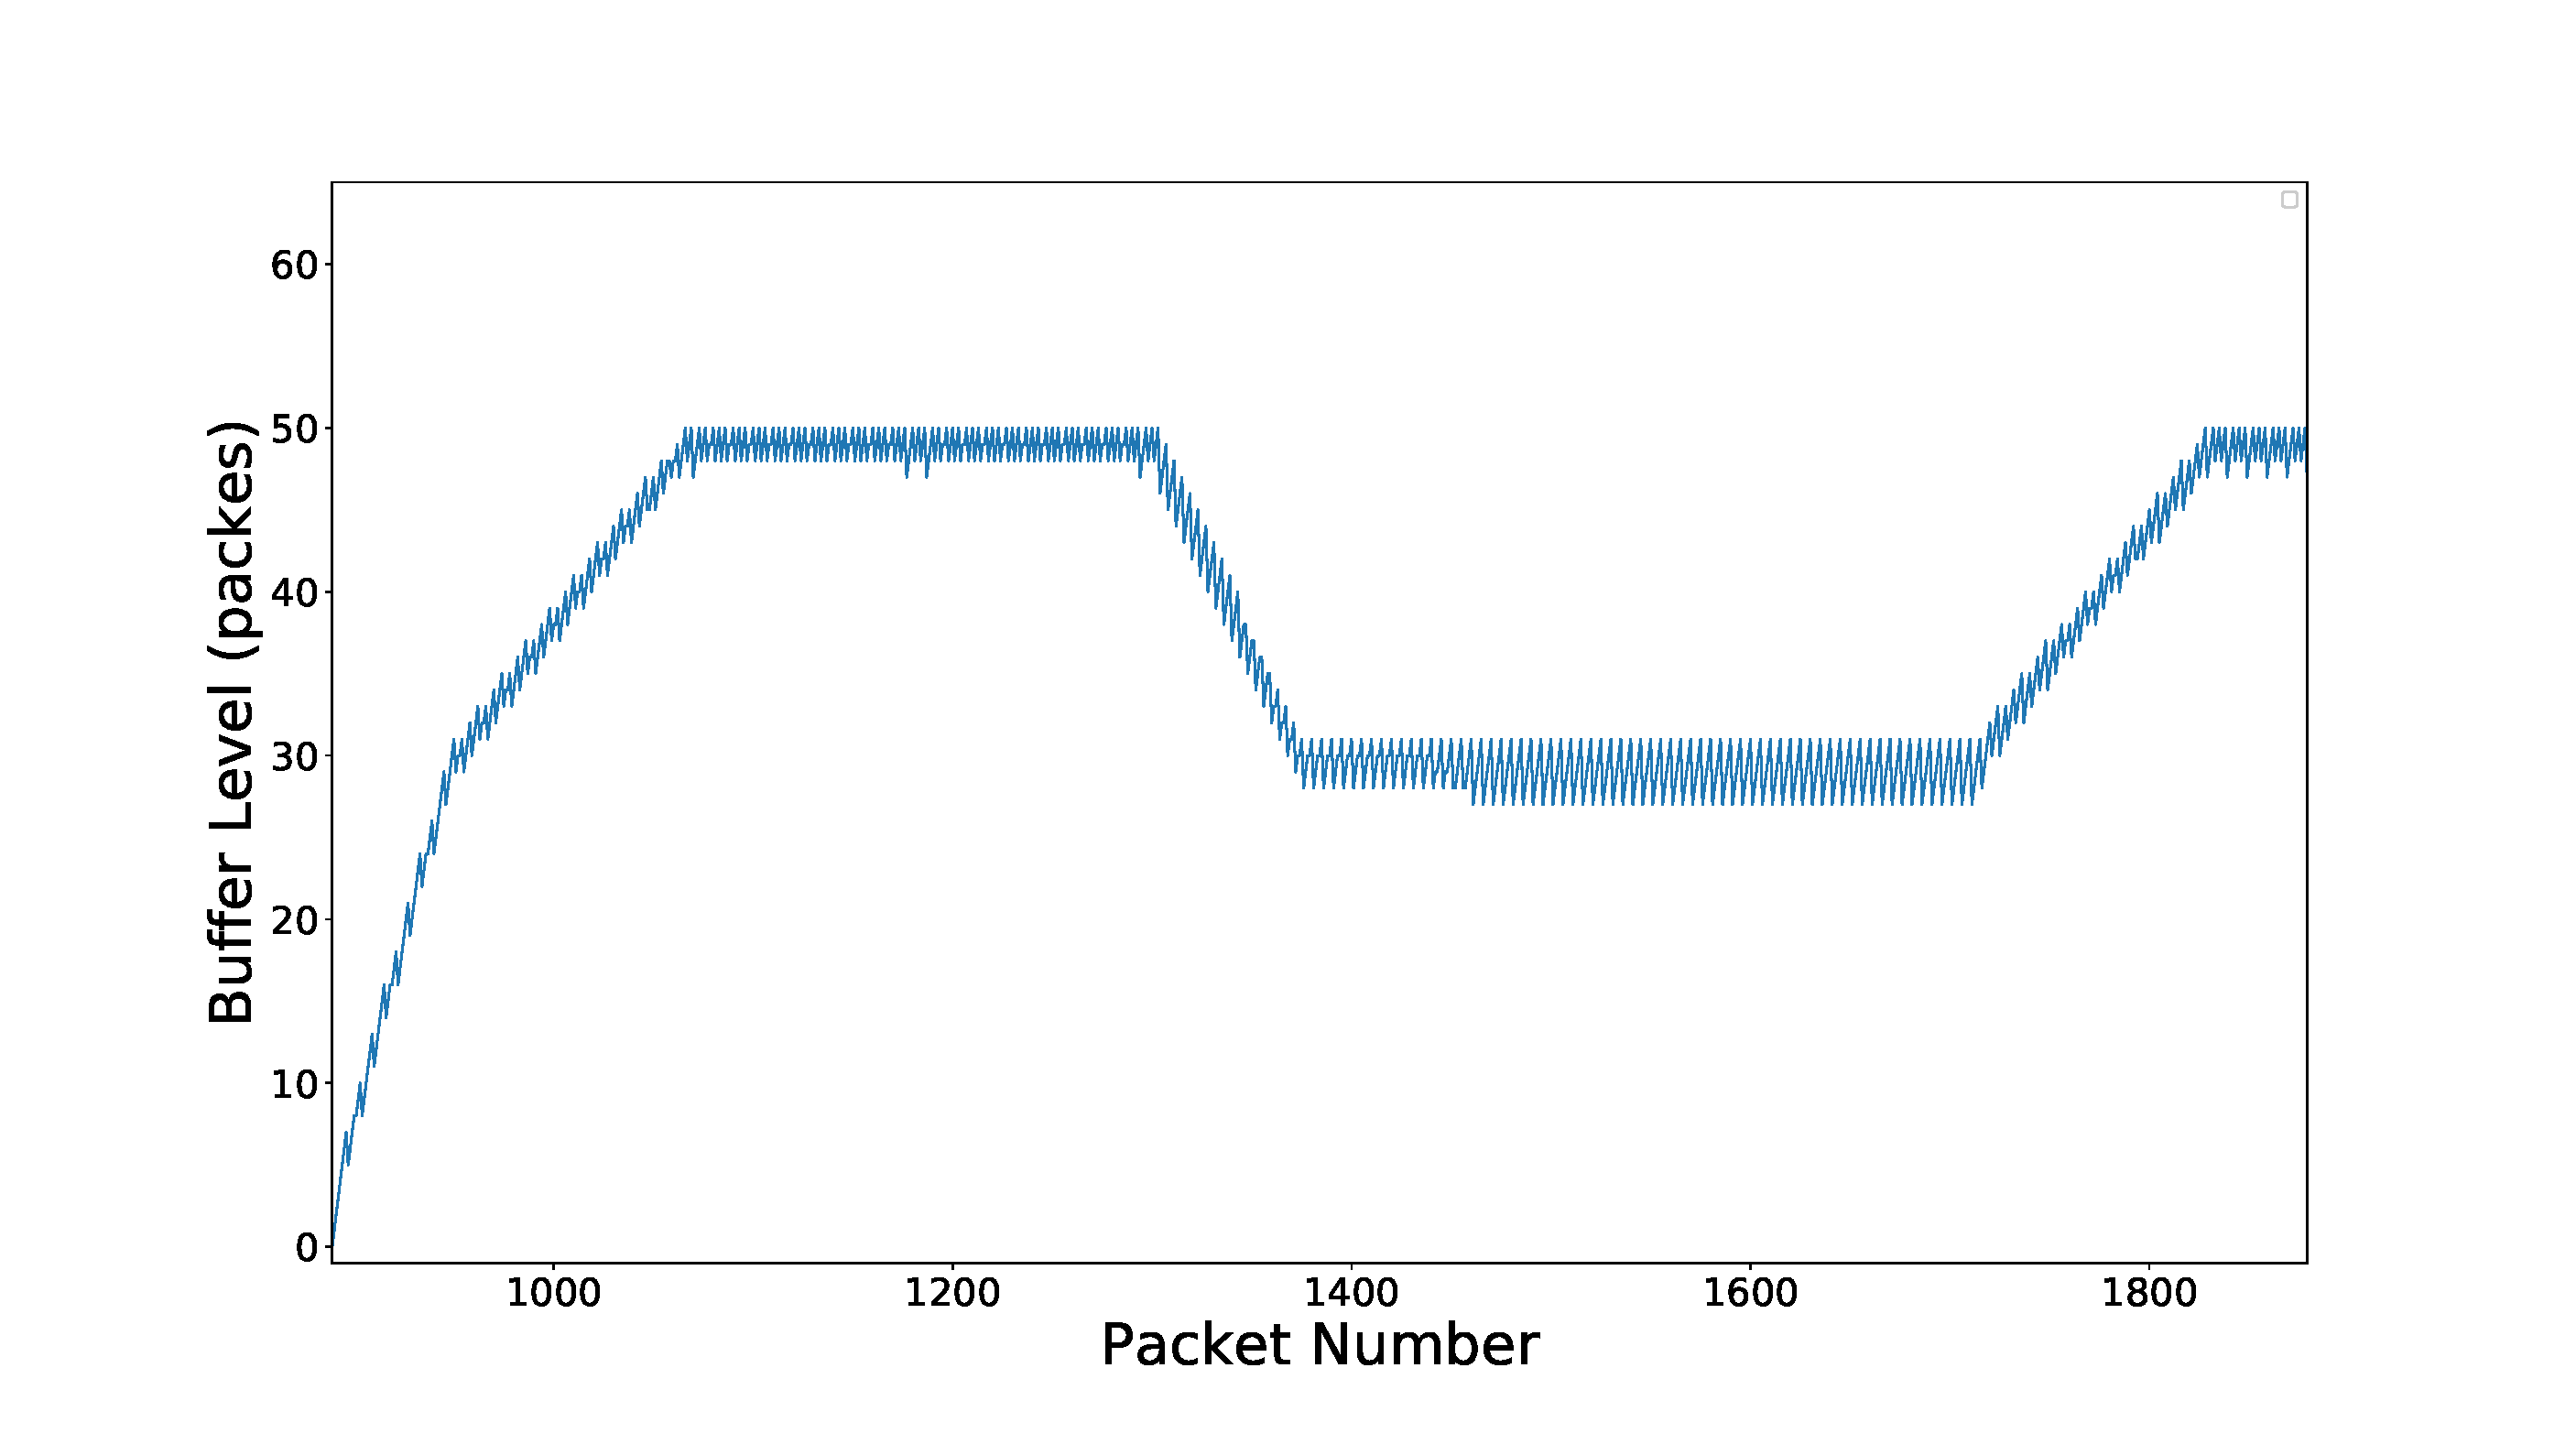
\includegraphics[width=\textwidth]{fig/EL_scenario3_buffer.eps}
        \caption{Buffer level of EL Logic in Scenario 3. (Flow 2)}
        \label{EL_buffer_level_S3_V2} 
        \end{minipage}
        \vspace{-0.1cm}
    \end{figure}
    %%%%


\end{subsection}

\section{Future Work} \label{sec:futureWork}

In our current implementation, we stream the video in SVEF which is using RDP only. However, this is not a good choice in real world. The scenarios we design only suit in experimental environments. Clients may want to receive a video content with lower quality instead of request a high quality video but receive something terrible. Furthermore, if the P4-based switch detect a network congestion. It should be able to send a message to server and reduce the sending rate. In the future, we will design an algorithm to adjust bitrate (sending rate) dynamically.

To implement this, we are going to use a SDN controller. Open Network Operating System(ONOS)~\cite{berde2014onos} is chosen because it is an  opensource project and it can work great with a P4 switch. ONOS is a modern SDN controller that provides some protocol, some applications, some tutorials, etc, and support by Google and Barefoot. There are already many SDN controllers and control protocols are using in the world. The reason we choose ONOS even it is still in development stage is that they design a new protocol for P4, P4Runtime~\cite{P4Runtime}.

As we mention above. There are already many protocols are used, should we design a new one? The condition is, if we design a protocol as we needed. There will just be one more alternative protocol. Therefore, ONOS provides a target independent, protocol independent, and pipeline independent protocol, which is P4Runtime. P4Runtime is a protocol for runtime control P4-defined switch. It provides protobuf-based APIs and automatically generates stubs for many languages. gRPC is a possible RPC transport. Moreover, this protocol won't change the P4 program running in the p4-target. In contrast, The target should provide a driver to tell ONOS how do they implement the pipeline and other architectures. Sometimes we want to use the controller to update P4 program or push new table into match+action table. P4Runtime also support this.

We design a topology to implement in the future. The network we design includes a sender, a controller, one Barefoot switch, three Raspberry Pi switches (with bmv2), and a receiver, as revealed in Fig.~\ref{scenario_3}. ONOS as a SDN controller is in charge of compiling P4 program and deploy to Barefoot switch and other RPis running bmv2. All the P4-target are also running P4Runtime to communicate with ONOS. All the links are Fast Ethernet cables. The bandwidths of links $d$ and $e$ are higher than the bandwidths of links $f$ and $g$. We physically remove link $e$ during streaming, and we expect to see that the ONOS controller reroutes the video stream through the Raspberry Pi 3 at the bottom. Because we configure links  $f$ and $g$ to have lower bandwidth, the video quality goes down. When we plug the Ethernet cable back, the ONOS controller reroutes the video stream over the Barefoot switch, and the quality of video stream goes up. 

\begin{figure}[tbh]
	\centering
	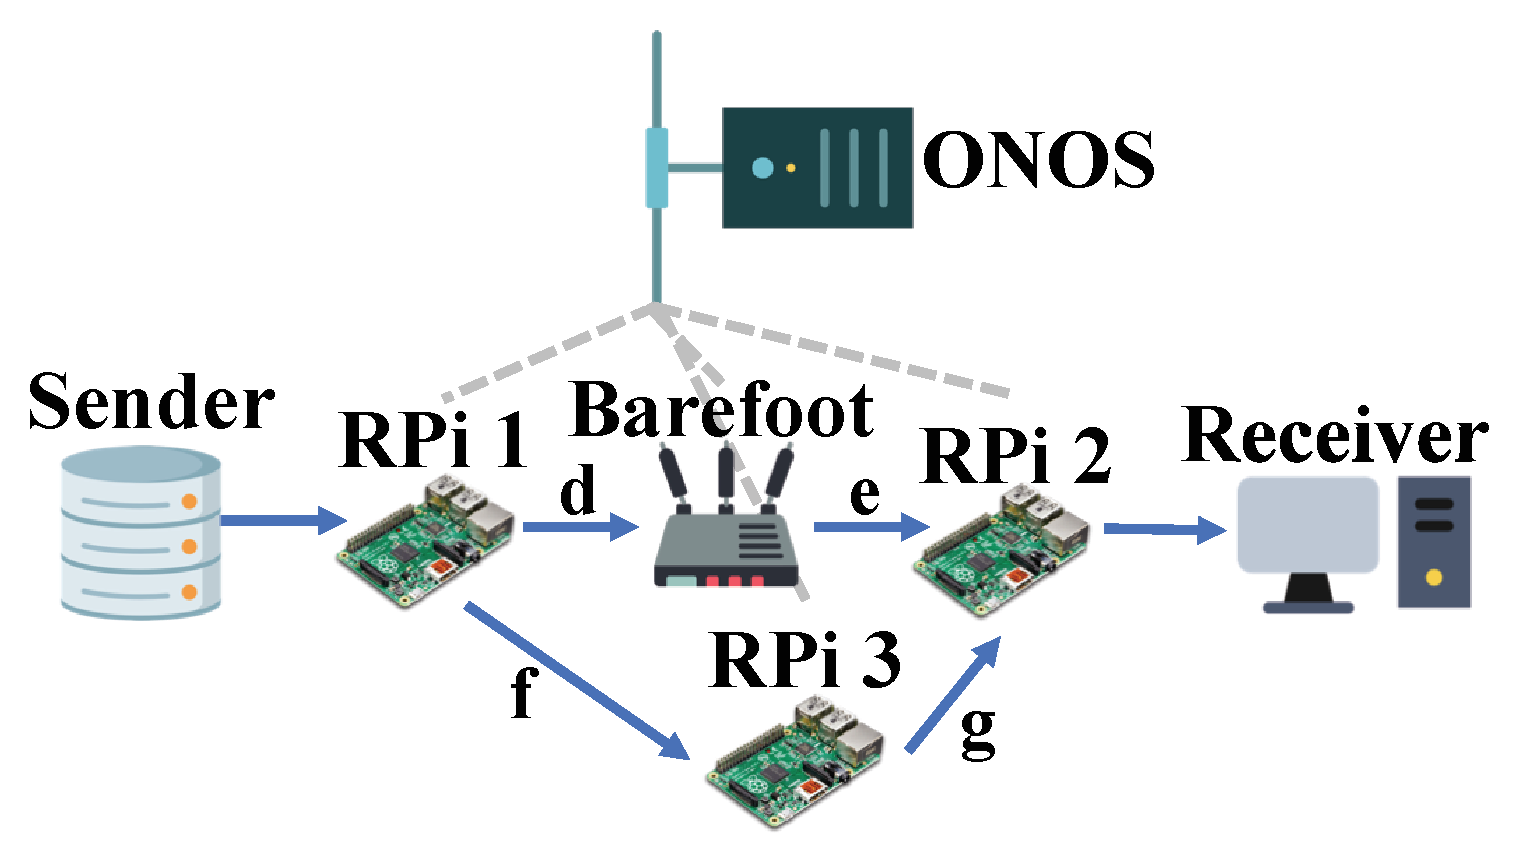
\includegraphics[width=.30\textwidth]{fig/scenario_3.eps}
	\caption{Future work Topology.}
	\label{scenario_3} 
\end{figure}
%\section{Research Problem} \label{sec:Remark Problem}

SVC can help us to reduce network congestions but selecting some proper layer to stream isn't a optimal solution. The network condition would change violently in runtime. Select the packets in middle of Internet would be much better than decide them in the beginning. Nevertheless, regular switches in the Internet can't drop any particular packets. The working logic of them is such easy as store and forward all the packets. The packets will be drop without any remedy in UDP protocol which is the most used protocol in video streaming. In SVC sequence, the higher layer can be decode depends on the lower layer. In other words, forwarding the higher enhancement layer without the lower enhancement layer waste the network resource a lot. 

To solve this problem, we are going to use {\em Programming Protocol-Independent Packet Processors (P4)} ~\cite{BDGI+14} programming language to design a switch to drop some useless packets in the middle of the Internet. P4 is a new describing language with following features. (i) Protocol Independent, (ii) Target Independent, and (iii) Field Reconfigurable. Protocol independent allows us to design any protocol we want to forward the packet, and thus we can add some user-specific field in the header for us to make our decision. Target independent allows us to describe everything from high-performance ASICs to software switches. Field reconfigurable allows us to change the way our switches process packets after we deploy our p4 program. 

\begin{figure}[tbh]
    \centering
    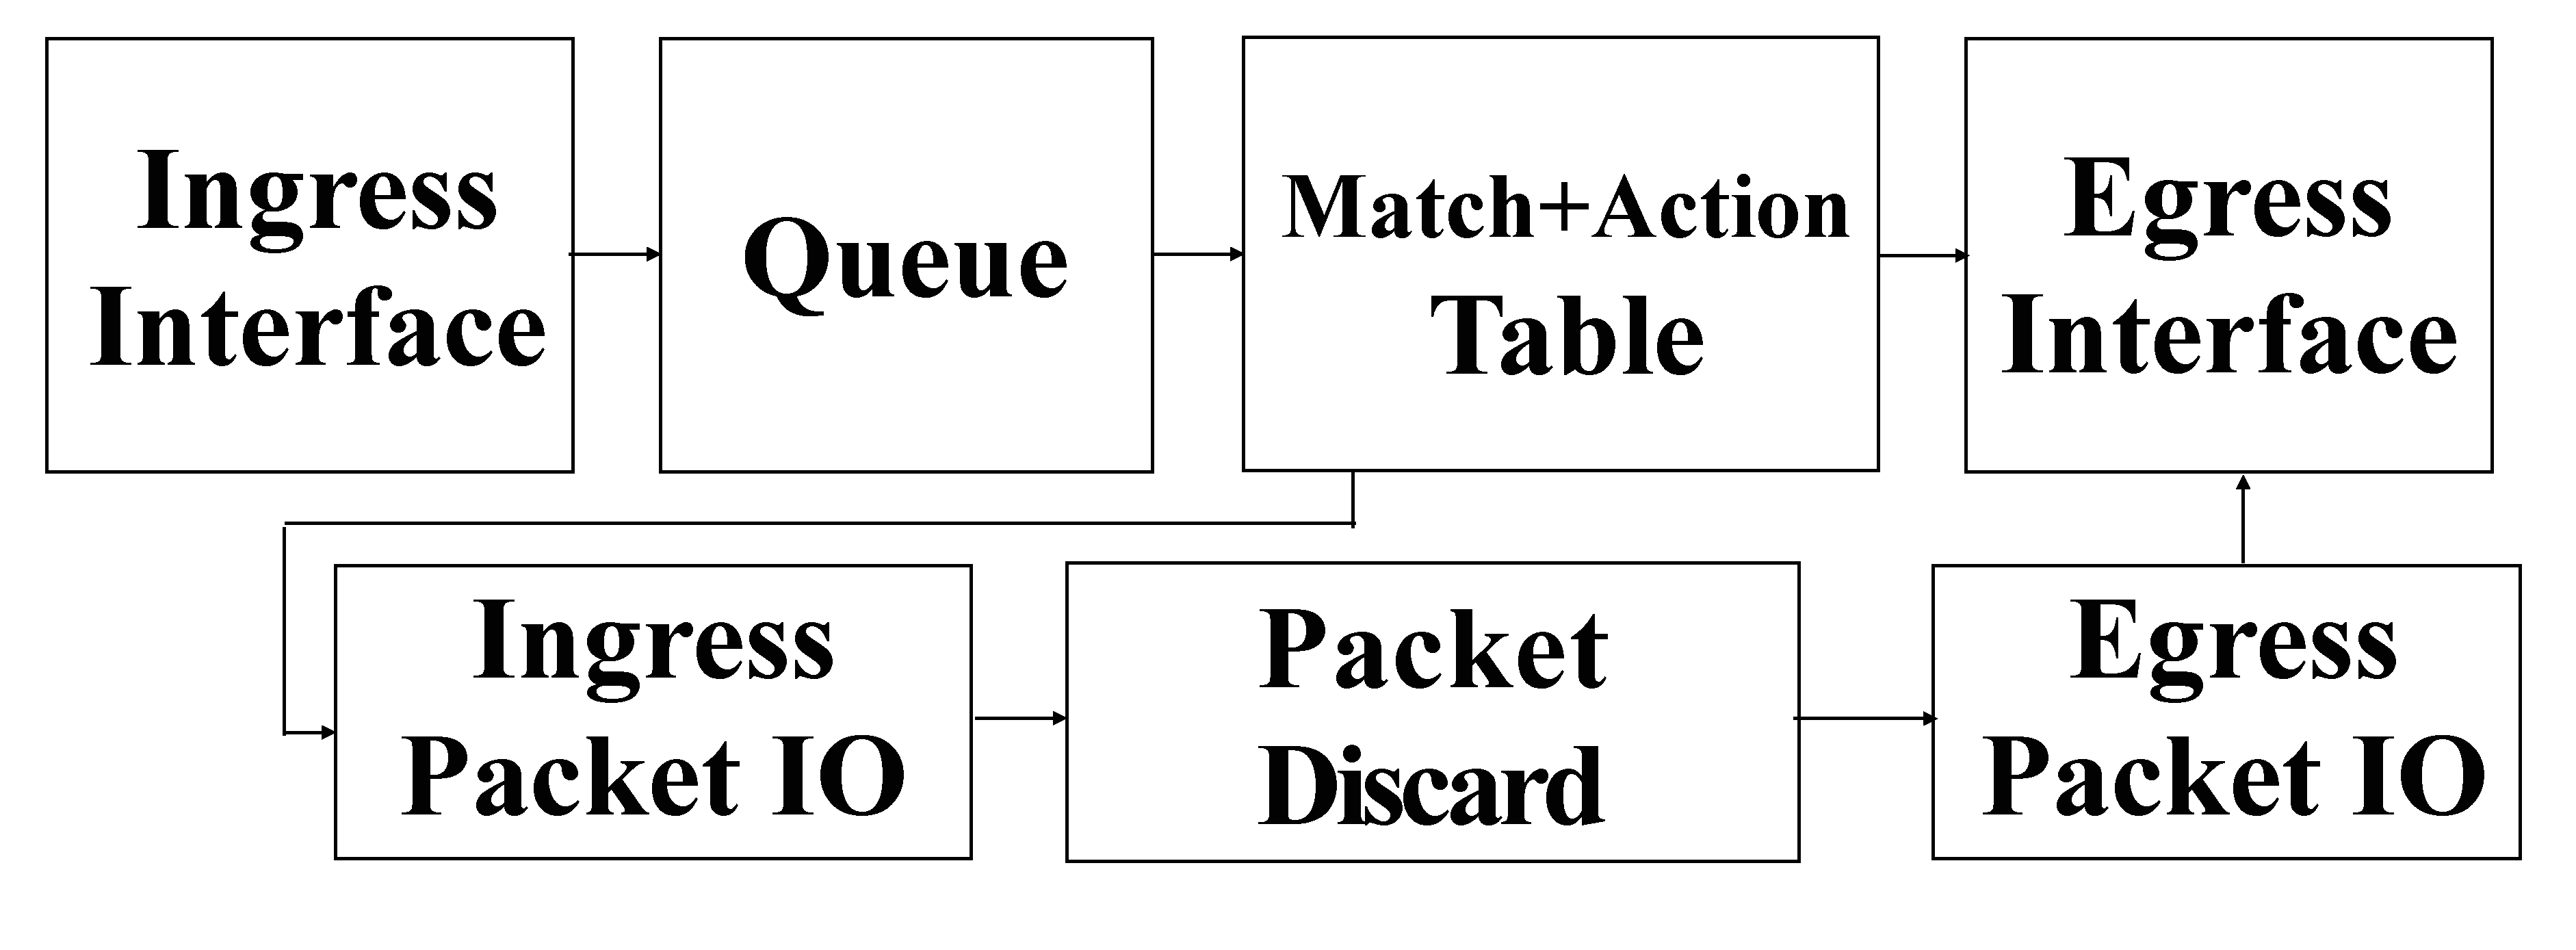
\includegraphics[width=.24\textwidth]{fig/MANE_1.eps}
    \caption{Packet processing in a P4-based MANE.}
    \label{MANE}
\end{figure}

Fig. ~\ref{MANE} shows how the P4-based MANE process packets. We define some header format and parsers which allow us to understand the structure of the packet. Incoming packets will first be parsed and divide into header and payload. We can design some match+action table in both ingress and egress control program to determine how to process the packet. In the ingress program, we can specify some match+action table to apply and may drop the packet if it's not valid or useless. After the packet pass the ingress program, it will be pushed into queues and than processed by the egress program. In P4, we can also calculate the checksum, configure forwarding table, construct some metadata adding to the header. With these tools and the knowledge of the whole Internet,  we can drop packets optimally in P4-based MANEs. 

On the other hand, P4-based MANE can not detect the condition of the whole Internet. Therefore, we combine P4-based MANE and SDN controller. Here we select {\em Open Network Operating System (ONOS)} to be our controller because it can from a controller plane without too many settings and it supports P4-runtime. P4-runtime is a program for controller to reconfig the P4-based MANEs. In other words, we can change the behavior of the P4-based MANE in runtime through P4-runtime. It works like a RESTful API server, we can simply give some commands to control our P4-based MANEs. 
%\section{Tentative Solution} \label{sec:Tentive Soution}

To drop scalable video packets to retain streamed video quality when bandwidth is in sufficient and dynamic. We plan to implement the following three drop logics. (i) Tail, (ii) Enhancement Layer (EL), and (iii) Rate-Distortion Optimize (RDO). Tail always drop the last packet while EL drops the enhancement layer packets.  The advantage of tail is the simplicity. EL ensure the decodability since we always forward the base layer packet. RDO takes the nature of rates between packet length and distortion into consideration, and than drop the packet with largest rate. Furthermore, we will record the frame number and layer id of the dropped packet. Therefore, we can also drop the other packets with the same frame number and higher layer id. RDO logic aims to minimize the negative impact of dropping packets. 

\begin{figure}[tbh]
    \centering
    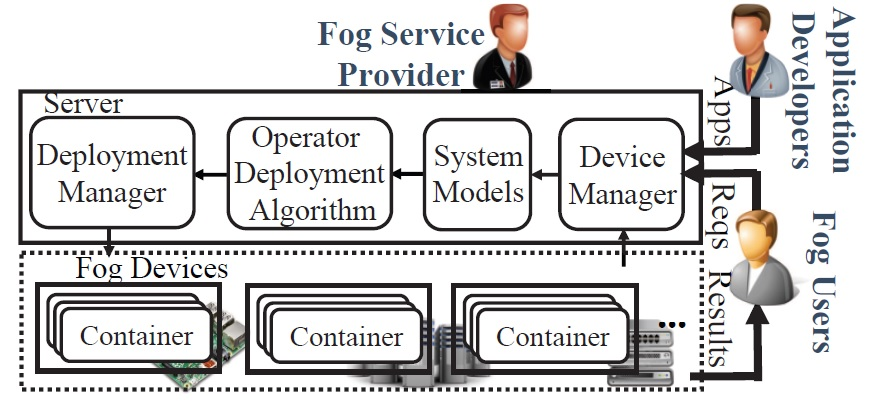
\includegraphics[width=0.40\textwidth]{fig/architecture.eps}
    \caption{High-level system architecture with a network of MANEs.}
\vspace{-0.1cm}
    \label{architecture} 
\end{figure}

Figure. ~\ref{architecture} show our architecture of the whole system. It is composed of a sender, some clients, some P4-based MANEs, some regular switches, and a ONOS controller connects those MANEs. The ONOS controller forms a control plane disassociate from the data plane. 

%\section{Expect Outcome} \label{sec:Expect Outcome}


%\section{Plan} \label{sec:Plan}

To approach our goal, we have learned how to write P4 programming language and setup our testbed inside Mininet. The next step is to finish our three drop logics, tail, EL, and RDO in our P4-based MANEs. Then we will run some experiments to make sure we optimally drop the packets. To leverage the advantage of SDN, we connect the P4-based MANEs with the ONOS controller. Next we will set up an server or write a program for developers to command our P4-based MANE in runtime, and we also need to make the controller able to reroute the flows if there's a physical disconnection.

%\section*{Acknowledgements}
%This work was partially supported by the Ministry of Science and Technology of Taiwan under the grant \#106-2221-E-007-101.
%\begin{figure}
%	\centering
%	\includegraphics[width=0.7\linewidth]{noms18Demo}
%	\caption{}
%	\label{fig:noms18demo}
%\end{figure}

%{\small
\bibliographystyle{abbrv}
\bibliography{./ref}
%}
\end{document}

